\documentclass[10pt, a4paper]{article}

\usepackage{amsmath}
\usepackage{amssymb}
\usepackage{fullpage}
\usepackage{algorithm2e}
\usepackage{graphicx}
\usepackage{wrapfig}



\newcounter{wssection}
\newcounter{wsexercise}[wssection]


\newcommand{\worksheetsection}[1]{
\vspace{10mm}
\stepcounter{wssection}
\noindent \Large \textbf{\thewssection. #1} \normalsize
\vspace{3mm}
}


\newcommand{\worksheetexercise}{
\stepcounter{wsexercise}
\vspace{5mm} \noindent \textbf{Exercise \thewssection.\thewsexercise \;}
}


\title{Dublin R Workshop on Time Series Analysis}
\author{Mick Cooney\\mickcooney@gmail.com}
\date{Autumn 2013}



\begin{document}

\maketitle


\worksheetsection{Basic Concepts}

\noindent
Time series occur in almost any field of study that produces
quantitative data. Whenever quantities are measured over time, those
measurements form a time-series, or more formally, a
\emph{discrete-time stochastic process}.

One reasonably famous example of a time-series is count of airline
passengers in the US, as seen in Figure \ref{fig1}. This is a fairly
simple time-series, with measurements taken on a monthly basis over a
number of years, with each datum consisting of a single number,
i.e. this time-series is \emph{univariate}.

\begin{figure}[h]
\begin{center}
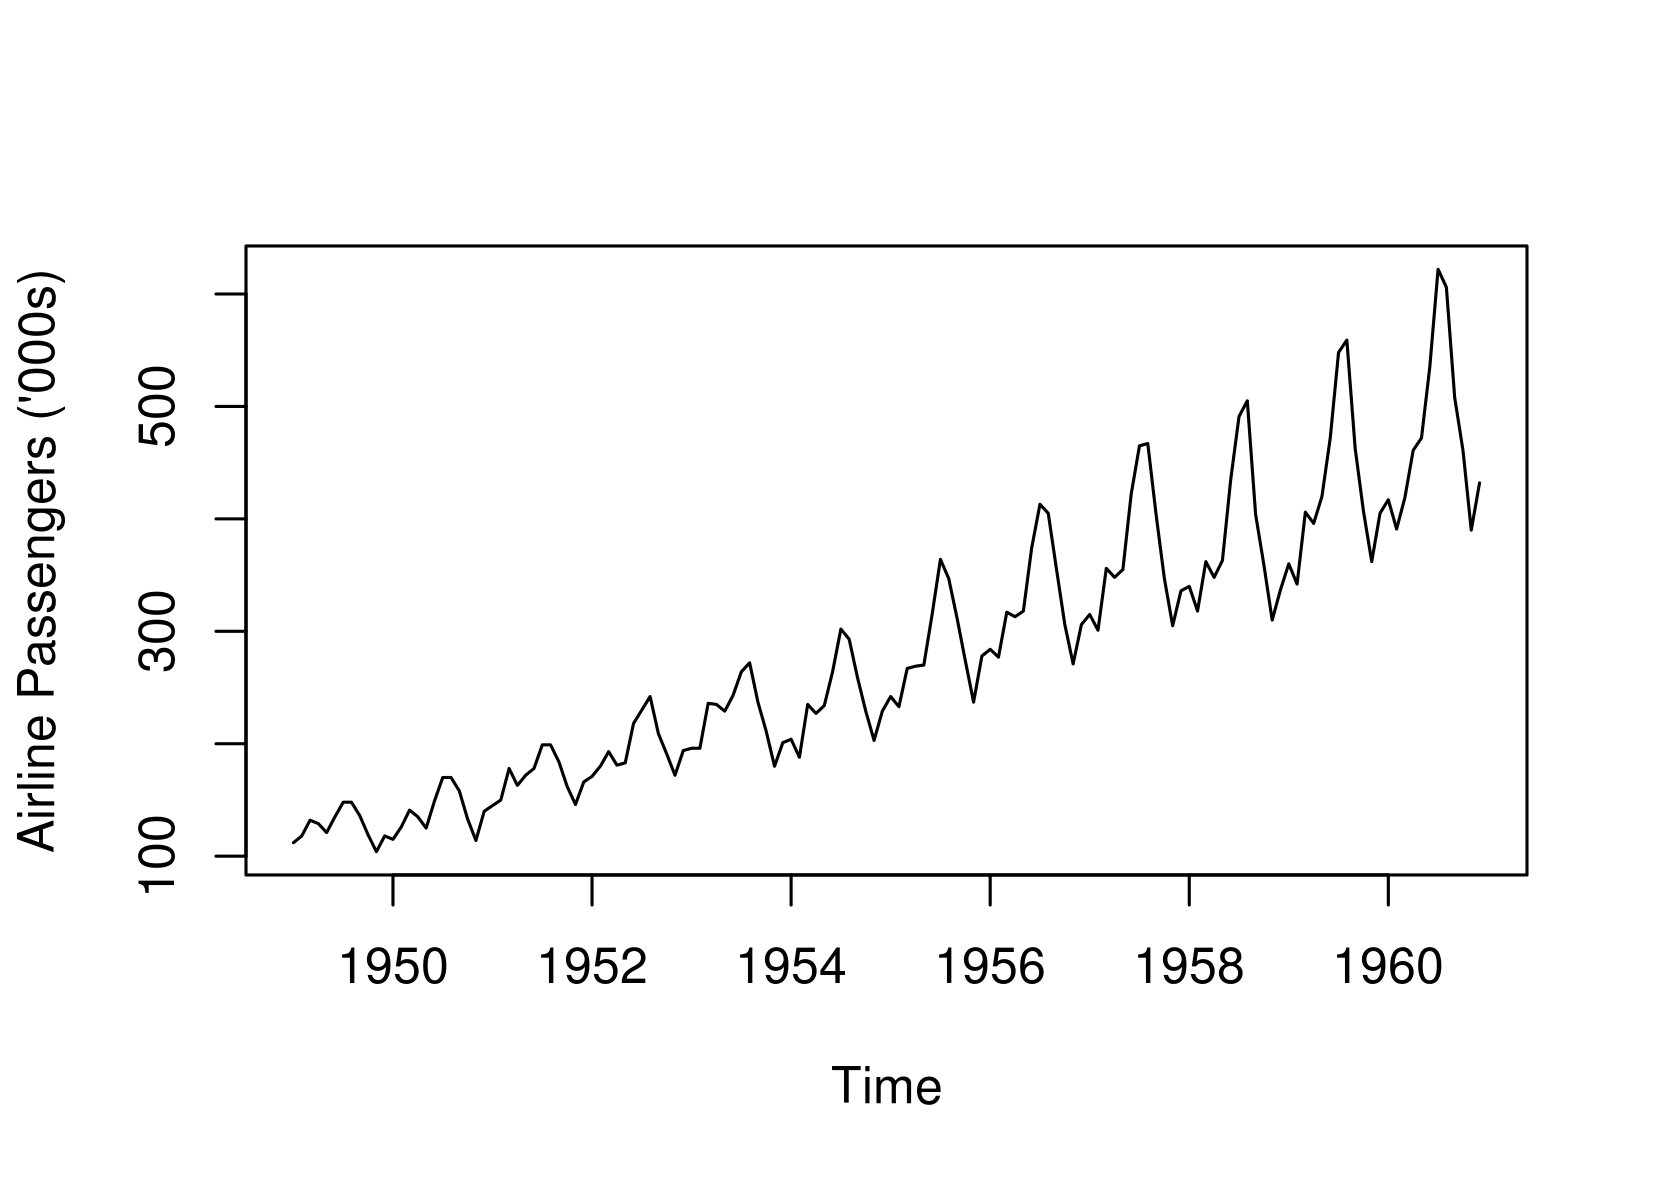
\includegraphics{airline_passengers_plot.png}
\caption{\label{fig1}
Example of a Time Series: Monthly Airline Passengers in the US}
\end{center}
\end{figure}


Before we begin trying to analyse data such as this, we need to first
create some kind of mathematical framework to work in. Fortunately, we
do not need anything too complicated, and for a finite time-series of
length $N$, we model the time series as a sequence of $N$ random
variables, $X_i$, with $i = 1, 2, ..., N$.

It is important to realise that each individual $X_i$ is a wholly
separate random variable --- analysing time series statistically is
unusual as we only ever have a single measurement from which we can
do inference. In many cases we simplify this much further, but it is
important to understand and appreciate that such simplifications are
just that, and this is often the reason why time series can be very
difficult to analyse.

Before we get to any of that though, and before we try to build any
kind of models for the data, we always start with visualising the
data. Often, a simple plot of the data helps use pick out aspects to
analyse and incorporate into the models. For time series, one of the
first things to do is the \emph{time plot}, a simple plot of the data
over time.

For the passenger data, a few aspects stand out that are very common
in time series. It is apparent that the numbers increase over time,
and this systematic change in the data is called the
\emph{trend}. Often, approximating the trend as a linear function of
time is adequate for many data sets.

A repeating pattern in the data that occurs over the period of the
data (in this case, each year), is called the
\emph{seasonal variation}, though a more general concept of `season'
is implied --- it often will not coincide with the seasons of the
calendar.

A slightly more generalised concept from the seasonality is that of
\emph{cycles}, repeating patterns in the data that do not correspond
to the natural fixed periods of the model. None of these are apparent
in the air passenger data, and accounting for them are beyond the
scope of this introductory tutorial.

\worksheetexercise
Load the air passengers data into your workspace and investigate the
structure of the \texttt{ts} object using \texttt{str()}. How is a
\texttt{ts} object different from a standard vector in R? Plot it
using the default \text{plot} method.

\worksheetexercise
Using the data supplied in the file \texttt{Maine.dat} and the
function texttt{read.table()}, load the Maine unemployment data into
your workspace and repeat the tasks above.

\worksheetexercise
Analyse the trend and seasonality for the air passenger data by using
the \texttt{aggregate()} function. Create a boxplot for the data,
segmenting the data by month.

\worksheetexercise
Repeat the above analysis for Maine unemployment data.





\end{document}
